\chapter[\texorpdfstring{bio2Byte Tools Deployment as a Python Package and Galaxy Tool to Predict Protein Biophysical Properties}{bio2Byte Tools Deployment as a Python Package and Galaxy Tool to Predict Protein Biophysical Properties}]{bio2Byte Tools Deployment as a Python Package and Galaxy Tool to Predict Protein Biophysical Properties.}\label{chapter:b2btools_deployment}
\chaptermark{b2BTools deployment}

Jose Gavalda-Garcia $^{1,2,\dag}$, Adrián Díaz $^{1,2,\dag}$, and Wim Vranken $^{1,2}$.
\\
\\
$^{1}$ Interuniversity Institute of Bioinformatics in Brussels, ULB-VUB, \\Brussels, Belgium.
\\
$^{2}$ Structural Biology Brussels, Vrije Universiteit Brussel, Brussels, Belgium.
\\
$\dag$ Authors contributed equally to this work.
\\
\\
DOI: 10.1093/bioinformatics/btae543
\vspace{1em}
\hrule
\vspace{1em}
\noindent Expanded for the thesis with work from: 
\begin{itemize}

\item Luciano Kagami, Joel Roca-Martínez, \textbf{Jose Gavaldá-García}, Pathmanaban Ramasamy, K. Anton Feenstra, and Wim F. Vranken. Online biophysical predictions for SARS-CoV-2 proteins. \textit{BMC Molecular and Cell Biology}, 22(1):23, April 2021.

\item Luciano Porto Kagami, Gabriele Orlando, Daniele Raimondi, Francois Ancien, Bhawna Dixit, \textbf{Jose Gavaldá-García}, Pathmanaban Ramasamy, Joel Roca-Martínez, Konstantina Tzavella, and Wim Vranken. b2bTools: online predictions for protein biophysical features and their conservation. \textit{Nucleic Acids Research}, 49(W1):W52–W59, July 2021.

\end{itemize}
\vspace{1em}
\hrule
\vspace{1em}
\begin{abstract}
We introduce a unified Python package for the prediction of protein biophysical properties, streamlining previous tools developed by the Bio2Byte research group. This suite facilitates comprehensive assessments of protein characteristics, incorporating predictors for backbone and sidechain dynamics, local secondary structure propensities, early folding, long disorder, beta-sheet aggregation and FUS-like phase separation. Our package significantly eases the integration and execution of these tools, enhancing accessibility for both computational and experimental researchers. \\
\textbf{Availability and Implementation:} The suite is available on the Python Package Index (PyPI): \href{https://pypi.org/project/b2bTools/}{https://pypi.org/project/b2bTools/} and Bioconda: 
\href{https://bioconda.github.io/recipes/b2btools/README.html}{https://bioconda.github.io/recipes/b2btools/README.html} for Linux and macOS systems, with Docker images hosted on Biocontainers: \href{https://quay.io/repository/biocontainers/b2btools?tab=tags\&tag=latest}{https://quay.io/repository/biocontainers/b2btools?tab=tags\&tag=latest}
and Docker Hub: \href{https://hub.docker.com/u/bio2byte}{https://hub.docker.com/u/bio2byte}. Online deployments are available on Galaxy Europe: \href{https://usegalaxy.eu/root?tool\_id=b2btools\_single\_sequence}{https://usegalaxy.eu/root?tool\_id=b2btools\_single\_sequence} and our online server: \href{https://bio2byte.be/b2btools/}{https://bio2byte.be/b2btools/}. The source code can be found at \href{https://bitbucket.org/bio2byte/b2btools\_releases}{https://bitbucket.org/bio2byte/b2btools\_releases}.


\end{abstract}

\section*{Aims of this chapter}
\begin{enumerate}
    \addtocounter{enumi}{2}
    \item Our research group, bio2Byte, has developed multiple tools to study different aspects of protein dynamics. While these tools provide complementary predictions of protein dynamics, unified execution was not possible at the start of this thesis due to incompatible requirements and syntax. Considering these limitations: 
    \begin{enumerate}
        \item Can we harmonise these tools into a unified suite to enable seamless execution?
        \item Can we improve the tools' deployment to ensure long-term usability and expand accessibility for users without programming proficiency?
    \end{enumerate}
\end{enumerate}

\section*{\textcolor{red}{Contribution to this work}}
\textcolor{red}{For the core of this work \cite{gavalda-garcia_bio2byte_2024}, I have closely collaborated with Adrián Díaz, with most tasks performed jointly. As examples, together, we unified dependencies and updated code when needed; I designed the python interface while Adrian designed the bash equivalent; I created the tests scripts to confirm the correctness of the results with every new version and he implemented their automatic execution prior to publishing; I wrote the plotting scripts for Galaxy Europe while he created the tool from the archived biocontainer. The most notable non-joint contribution in this work is the updating of the machine learning models to newer versions, which is rarely supported by the required packages and required extensive work to understand and convert to the required model file format.}

\textcolor{red}{Regarding the articles used to expand the chapter \cite{kagami_online_2021, kagami_b2btools_2021}: For the article on SARS-CoV-2, I participated in selecting homologous proteins, creating MSA, and generating and formatting of the predictions, in addition to writing the corresponding section of the manuscript and testing the web resource. For the article on b2BTools server deployment, I directly contributed to the update of the tools}



\newpage
\section{Introduction}

Proteins are complex molecules whose motions often play a fundamental role in their function \cite{fenwick_integrated_2014, campbell_role_2016}. The experimental study of the dynamics of proteins offers insights on properties such as order and flexibility, folding mechanics, conformational changes and secondary structure populations \cite{berjanskii_nmr_2006, eaton_modern_2021}. Such experiments, often using Nuclear Magnetic Resonance (NMR), provide valuable protein dynamics information but are expensive and time consuming with no high throughput possible. To obtain \gls{proteome}-scale estimations of such characteristics, predictors are essential, for example to examine trends between how expressable protein fragments are and their dynamics \cite{boone_massively_2021}, or to inform protein early folding characteristics in relation to experiments  \cite{smets_evolutionary_2022}.

We developed an assortment of predictors of protein properties that work from single amino acid sequences, encompassing estimations of backbone dynamics \cite{cilia_protein_2013, cilia_dynamine_2014}, early folding \cite{raimondi_exploring_2017} and long disorder \cite{orlando_prediction_2022} among others. The code for these tools was often developed separately, illustrating the natural progression of scientific software, with each tool originally employing its own contemporary dependencies and programming language versions. Though the code was openly available and each tool could be individually compiled with the precise set of dependencies' versions described in their repositories, this effectively requires a separate environment per tool and, potentially, significant effort to make each tool work. This contrasts with the complimentary nature of these tools, which together offer a more holistic vision of a protein's (dynamic) nature.

Here we present the progression on our tools' deployment from their original published deployment from their published source code to their unified deployment as a single Python package that can be employed on any Linux or macOS machine. The deployment protocol that we have defined publishes the package on the Python Package Index (PyPI) \cite{pypi} and Bioconda, the biomedical research channel of Conda package manager (only for Linux 64-bit and AArch64 or macOS x86 64)\cite{gruning_bioconda_2018}. In addition, it archives on Biocontainers \cite{da_veiga_leprevost_biocontainers_2017} to ensure reproducibility and publishes it on Galaxy \cite{afgan_galaxy_2018} Europe to enable its incorporation into pipelines and facilitating non-programmatic usage (process overview in \figref{overview_figure}). 

\section{SARS-CoV-2 Viral Proteins Database}

The first work featuring a unified presentation of our tools' outputs was a reaction to the SARS-CoV-2 health emergency. The pandemic highlighted the need for rapid and accessible computational tools to aid in the global effort for treatment development. To address this, we developed a unified platform that presents our tool outputs in a user-friendly manner. Although these tools were publicly available as executable programs, we recognised that their diverse dependencies and syntax could be challenging for some researchers, particularly those with limited computational expertise. To overcome this, we processed all viral proteins with our tools, predicting their dynamic properties and aligning their homologs to SARS-CoV-2 proteins. The results were then calculated and presented within what we defined as each protein's ``biophysically-allowed space'' — the range of biophysical values permissible at each position of the alignment. Amino acids with a wider biophysically-allowed space are considered more permissible to changing biophysical behaviours to those with narrower spaces. Consequently, treatments targeting proteins at positions within a narrow biophysically-allowed space may be more effective, as such interventions could significantly alter protein behaviour.

The comprehensive database containing all results is available on our website (\burl{https://bio2byte.be/sars2/}) \cite{kagami_online_2021}. This resource includes interactive plots with the tool's results for each protein, the calculated biophysically-allowed space, and links to relevant entries in UniProt \cite{the_uniprot_consortium_uniprot_2023}, PDBe \cite{armstrong_pdbe_2020}, and NCBI \cite{sayers_database_2021}. Therefore, the data indicate protein behaviours in SARS-CoV-2 that are not evident from static structures, highlighting potential targets for disrupting protein function based on conserved biophysical characteristics, as shown by narrow ranges in their biophysically-allowed spaces. Additionally, this work revealed the complexity involved in the unified execution of our tools, which contrasted with the otherwise complementary nature of their outputs.

\section{Creation of bio2Byte Tools Web Server}

To facilitate the use of our tools, we developed a web server capable of executing a selection of them simultaneously (\burl{https://bio2byte.be/b2btools/}) \cite{kagami_b2btools_2021}. This server enables users to easily run a collection of tools by uploading a FASTA file through a user-friendly web interface, significantly lowering the computational skills required to utilise our tools. To support more advanced applications and seamless integration into pipelines, we also incorporated a token-based Application Programming Interface (API) into the server’s design. An API is a set of rules and protocols that enables different software systems to communicate with each other. This feature allows third-party software (\textit{e.g.} scripts retrieving protein information from multiple services and databases) to submit jobs and request results as part of their workflow. The API provides results in Comma-Separated Values (CSV) or JavaScript Object Notation (JSON) formats, which are machine-readable and easily integrated into subsequent processes. Moreover, these result files can be downloaded through the web interface using their token identifier, regardless of whether the job was submitted via the web interface or the API. Similarly, jobs submitted through the web interface can also be accessed and downloaded using the API, provided the token is available.

While deploying the web server provides convenience for many users, it also has certain drawbacks and limitations. One of the most significant drawbacks is that the execution of our tools depends on the availability of our service. If the server were to be permanently shut down, users would only be able to execute the tools from the published source code and environment descriptions, as was the case before the deployment of the web server. Additionally, each job submitted to the server is limited in size and subject to a queue, which is necessary to manage the server's computational resources effectively. This makes the web server approach less suitable for large-scale analyses and its dependency on server availability reduces the robustness needed for seamless integration into pipelines. To address these limitations, we also deployed bio2Byte Tools as a Python package, which allows users greater flexibility and overcomes the constraints associated with the web server.


\section{Tools Harmonisation and Packaging}
The tools included in this version of bio2Byte Tools were primarily sequence-based predictors, namely DynaMine \cite{cilia_protein_2013}, DisoMine \cite{orlando_prediction_2022}, EfoldMine \cite{raimondi_exploring_2017}, AgMata \cite{orlando_accurate_2020} and PSPer \cite{orlando_computational_2019}, which can estimate an array of metrics from a simple FASTA file, but also includes ShiftCrypt \cite{orlando_shiftcrypt_2020} for residue-level interpretation of NMR Chemical Shift data for proteins (Supplementary Table 6.1, \figref{fig:output_example}). 
% (\supptableref{tab:tool_explanation}, \figref{fig:output_example}).
Here, we focus on the description and integration of the sequence-based predictors, which facilitates their deployment in a single environment. The steps described in this work result in further FAIRification of our tools \cite{wilkinson_fair_2016}, now robustly available for the scientific community.

\begin{figure}[tbh]
    \centering
    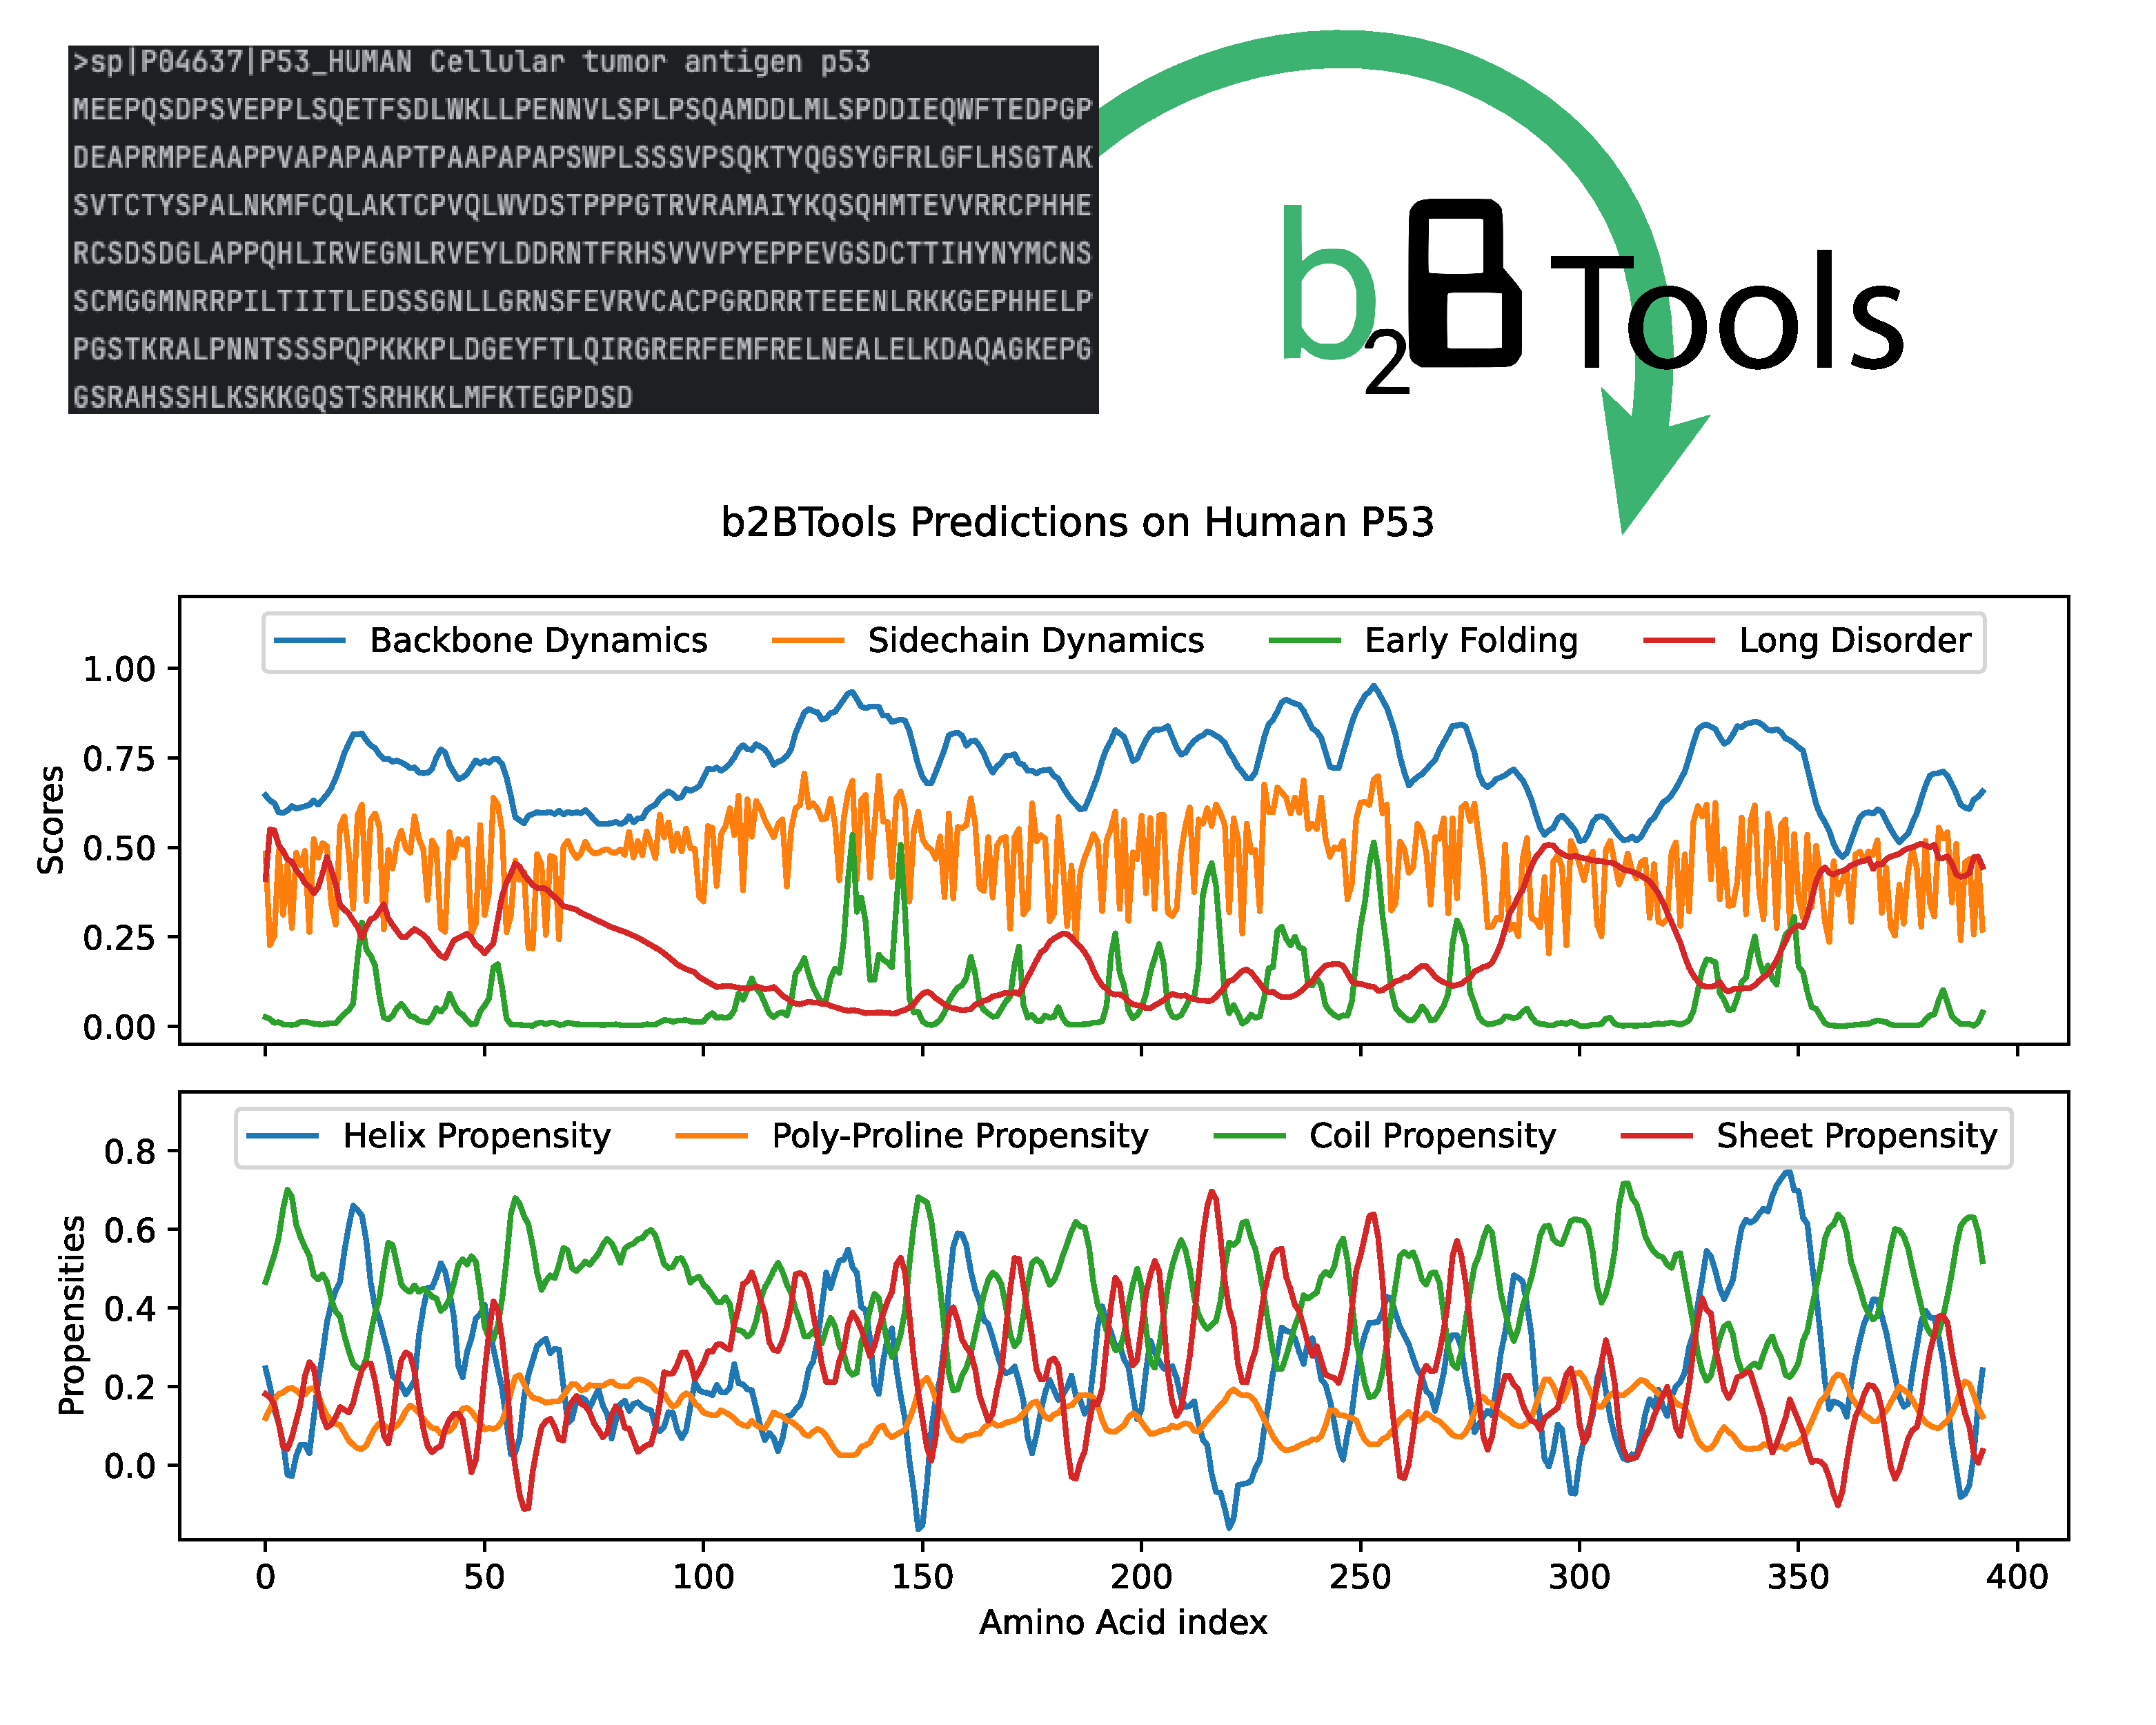
\includegraphics[width=1\linewidth]{b2b_deployment//Fig/output_figure_v2.pdf}
    \caption{\textbf{Execution of b2BTools on Human P53 protein.} Visual workflow showing the execution of b2BTools for a single protein in FASTA format. A selection of estimated biophysical values for this protein have been plotted on the right hand side of the figure.}
    \label{fig:output_example}
\end{figure}



\subsection{Code and Models Updating}
The fundamental first step to transform a set of tools into a suite was to unify all the dependencies. The code of all tools was updated to adopt syntax compatible with all Python versions between Python 3.7 and 3.12 and the deprecated calls to objects in external dependencies were substituted for current code with equivalent behaviour. Notably, the machine learning model files of these tools had to be updated to match the format of the updated dependencies, an action that is not recommended by the employed machine learning libraries (Scikit-learn \cite{scikit-learn} and PyTorch \cite{paszke_pytorch_2019}) and therefore, no standard model conversion procedure exists. This step required extensive labour to understand the old and updated model description file formats, to then update the trained model files. Given the risk to change the output of the tools, thorough tests were implemented in a diverse set of proteins. This ensured that the difference in outputs between legacy and unified tools was no larger than floating point errors.

\begin{figure*}[!t]%
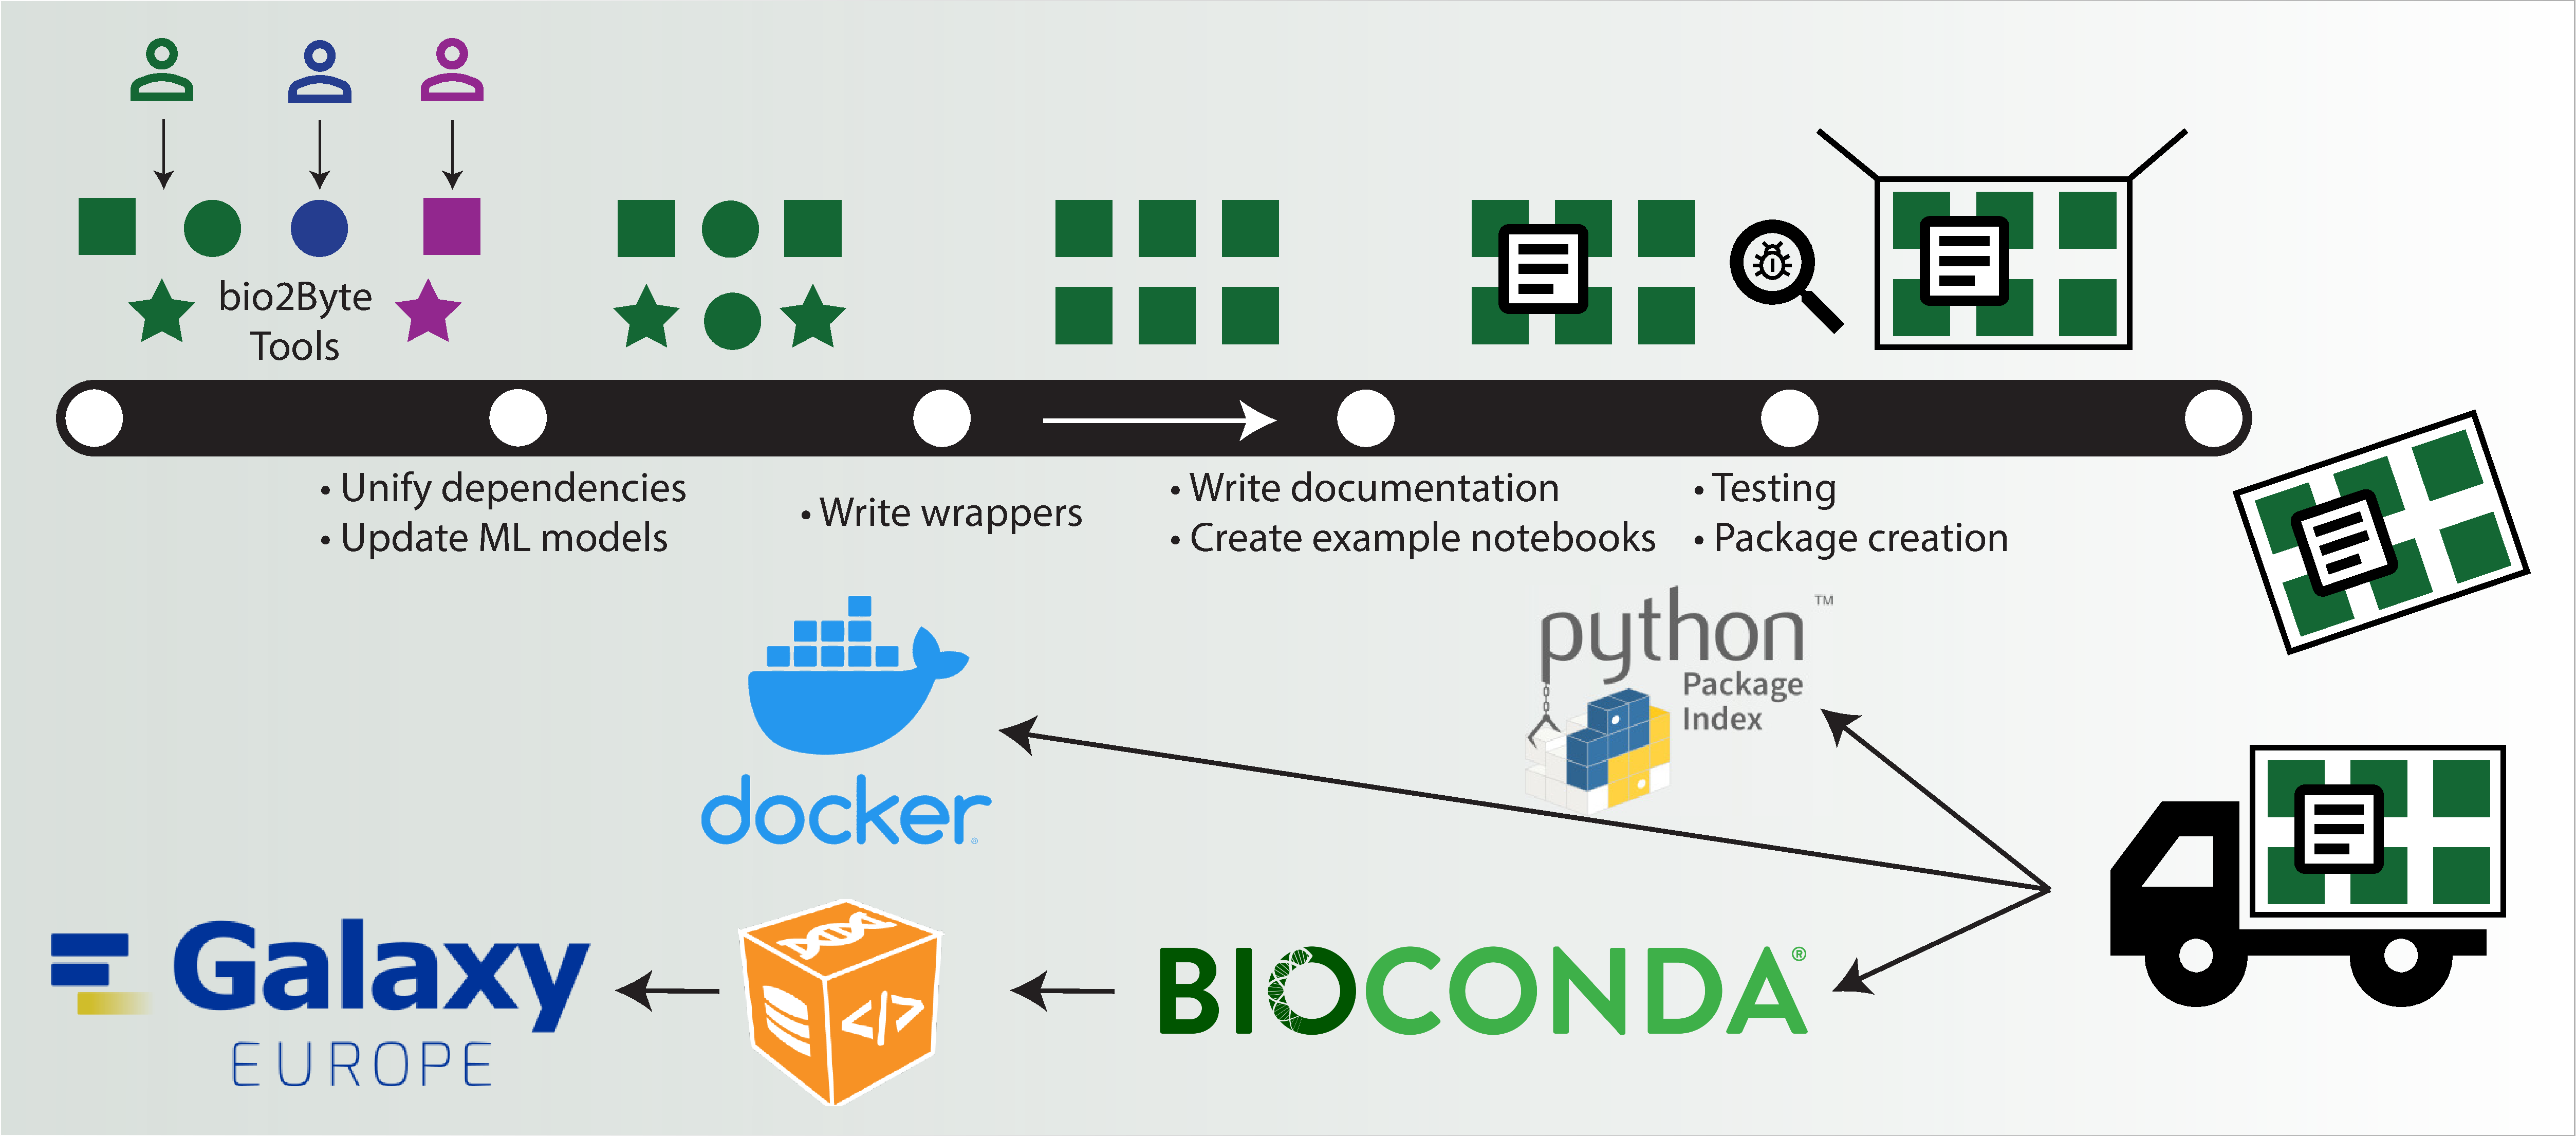
\includegraphics[width=\linewidth]{b2b_deployment/Fig/overview_slim.pdf}  
\centering
\caption{\textbf{Overview of the update and deployment process applied to bio2Byte Tools.} Even within a single research group, the development of tools over time and across various developers carries variation in dependencies and coding conventions, illustrated in the heterogeneous shapes and colours for the original softwares (top left). These tools have to go through a (figurative) production line to become a harmonised software package, during which the different tools acquire compatible shapes and colours. Once the tools fit together, a user manual, an extensive README.md and example notebooks can be included. Finally, quality is assured in the form of thorough execution and outputs tests and the package with all the harmonised tools can be created. This package leaves the production line and is deployed to different distribution channels and archived for ease of use and reproducibility.}
\label{overview_figure}
\end{figure*}

\subsection{Programmatic Usage and Execution}

To facilitate the execution of the predictors inside the package, their inner classes and methods were abstracted in a public wrapper class, named ``\textit{SingleSeq}'' and illustrated in code snippet \ref{single_seq_snippet}, which is the entry point for the users and acts as the interface between them and our predictors. This wrapper allows an easy parse of sequences in FASTA format, execution of the desired tools, storage for the outputs as a Python object dictionary, and export outputs and metadata as a JSON, CSV or TSV file (exemplified in code snippet \ref{single_seq_snippet} for Python usage and code snippet \ref{single_seq_snippet_bash} for bash usage). \textcolor{red}{The harmonisation of these tools into a unified suite in this thesis' aim 3-a is therefore fulfilled.} An equivalent wrapper is also available to execute the tools on a multiple sequence alignment (MSA), named ``\textit{MultipleSeq}'' and described in README.md, which maintains the aligned position of the amino acids and returns the bio2Byte Tools outputs indexed according to this alignment.


\begin{lstlisting}[caption={\textbf{Python execution of bio2Byte Tools.} This code will store for each individual sequence contained in \textit{example.fasta} a \textit{.json} output file with the predictions of the selected tools and their dependencies.}, label={single_seq_snippet}, float] 
import json
from b2bTools import SingleSeq

input_fasta = "/path/to/example.fasta"

single_seq = SingleSeq(input_fasta)
single_seq.predict(tools=["disomine"])
preds = single_seq.get_all_predictions()

for seq_id, pred_vals in preds["proteins"]:
    with open(f"{seq_id}.json", "w") as fp:
        json.dump(pred_vals, fp)
\end{lstlisting}

\begin{lstlisting}[language=bash, caption={\textbf{Bash execution of bio2Byte Tools.} This code will store the output of all sequences in the \textit{.fasta} input in \textit{.json} and \textit{.csv} files and will also store the metadata in a different file.}, label={single_seq_snippet_bash}, float] 
b2bTools \
  --input_file /input/example.fasta \
  --output_json_file /output/example.json \
  --output_tabular_file /output/example.csv \
  --metadata_file /output/example.meta.csv
\end{lstlisting}

To optimise resources, when a user selects the set of tools to run, their interdependencies are assessed (Supplementary Table 6.2)
% (\supptableref{tab:tool_dependencies})
and all required tools will be executed only once in the necessary order. For example, if DisoMine and DynaMine are selected for execution, DynaMine will run first, then EfoldMine (a requirement for DisoMine) and finally, DisoMine. In contrast, the legacy code would execute multiple instances of DynaMine, for each tool that depended on it. 

% \hl{[TODO: We need a big figure which contains the interdependencies of the tools as well as the different distributions and deployment]}

\subsection{Testing and Publishing}

Our tools were then contained in a Python package. With every new version, this package is subject to exhaustive unit tests using the library \lstinline|pytest| \cite{pytestx.y} to ensure codebase integrity and predictions consistency, \textit{i.e.} we assert that the code modification does not alter the predictor's outputs. 
We have automated the building and testing process by including a CI/CD pipeline in the package repository on Bitbucket. We run in parallel all the unit tests for every compatible Python version. Then the pipeline builds the Python package and tests its command-line execution with a simple FASTA input file (Supplementary Fig. 6.1).
% (\suppfigref{pytest}).

If all tests are successful, a new version is manually published on PyPI and Bioconda, which additionally tests that all modules and sub-modules can be correctly imported and called. Once these tests are passed, the new version of bio2Byte Tools get incorporated in Bioconda's index. As soon as this new version is included in Bioconda's index, a new \gls{dockerimage} is automatically built and published on the Biocontainers containers registry. 
This image on Biocontainers is created only for Python 3.10, so we also create a set of Docker images for each new version in three different flavours for each Python from 3.7 to 3.12 (Supplementary Table 6.3).
% (\supptableref{tab:docker_versions}). 
Each of these containers are subject to an additional iteration of the previously described unit tests upon creation. This ensures system-independent execution and reproducibility of results for every version of our software.

\section{Deployment in Online Pipelines}
With the software available online as a Python package and as a Docker image, we uploaded it as a tool on \gls{galaxyeurope}. This enables its usage in this platform as a standalone tool or as part of a workflow with other tools. The creation of the Galaxy package required the definition of the tool's user interface, which then defines all necessary settings to run our tools. This user interface allows code-free execution and, if selected, plotting of its outputs. \textcolor{red}{This ensures long-term usability for users with diverse levels of programmatic literacy, thereby fulfilling aim 3-b of this thesis.}

\section{Future Perspectives}

The docker image of bio2Byte Tools can now be deployed on our own server \cite{kagami_b2btools_2021}, and will soon substitute the original custom and more convoluted approach with multiple environments. 

Furthermore, one of the most anticipated features under development for this software suite is the creation of a protocol for Nextflow \cite{di_tommaso_nextflow_2017} so that our tools can be easily incorporated and shared as part of reproducible pipelines. \Gls{nextflow} also allows for easy scaling of the workload among all available processing units, effectively accelerating the calculation of large data sets. 

Additionally, though this suite is able to use evolutionary information from an MSA to estimate the biophysical constraints of residue positions in a protein family, it does not provide additional interpretation of such results. We are currently working on an extra layer of interpretation for such information, for example to determine how well a protein fits within those biophysical constraints. 

We will continue to update the suite as new Python versions are released, aiming to maintain support for older versions whenever possible. Finally, we hope the improved usability and reproducibility of our tools will encourage its further incorporation in scientific resources.


\section*{Additional Resources for bio2Byte Tools}

An extensive collection of example notebooks can be found on \url{https://github.com/Bio2Byte/public_notebooks/}, which will reflect future updates and new functionalities of our suite.

\section*{Supplementary Information}
Supplementary information for this work can be found on Zenodo following this url: \burl{https://zenodo.org/doi/10.5281/zenodo.13621734}.

\section*{Author Contributions}
J.G.-G. and A.D. developed, implemented and validated the software suite and CI/CD pipelines.
W.V. provided supervision and implemented the initial integrated version of the prediction tools.
All authors contributed to the writing of the manuscript.

% Regarding the articles used to expand the chapter: For the article on SARS-CoV-2, I participated in selecting homologous proteins, creating MSA, and generating and formatting of the predictions, in addition to writing the corresponding section of the manuscript and testing the web resource. For the article on b2BTools server deployment, I directly contributed to the update of the tools.

% \section*{Conflicts of Interest}
% The authors declare no conflict of interest.

% \section{Author contributions}
% J.G.-G. and A.D. developed, implemented and validated the software suite and CI/CD pipelines.
% W.V. provided supervision and implemented the initial integrated version of the prediction tools.
% All authors contributed to the writing of the manuscript.

